%! Author = mariuszindel
%! Date = 02.11.20

\section{gRPC (Remote Procedure Call)}

\subsection{Überblick}
\begin{itemize}
    \item Neue Standard-Technologie für Backend-Kommunikation in .NET
    \begin{itemize}
        \item Primär Server-to-Server Kommunikation im Fokus
        \item Hohe Performance von zentraler Bedeutung
        \item Nicht als Frontend-API gedacht
    \end{itemize}
    \item Basistechnologien
    \begin{itemize}
        \item Kommunikationsprotokoll: HTTP/2
        \item Interface Definition Language IDL: Google Protocol Buffers
    \end{itemize}
    \item Löst Probleme wie:
    \begin{itemize}
        \item Security
        \item Syncronisation
        \item Data Flow Handling
    \end{itemize}
    \item GrundPrinzipien:
    \begin{itemize}
        \item Einfache Service-Definition
        \item Sprach-Unabhängig
        \item Problemlose Skalierbarkeit
        \item Bi-direktionales Streaming
        \item Integrierte Authentisierungsmechanismen
    \end{itemize}
    \item Fast alle Sprachen werden unterstützt (Java, C++, Python, etc.)
\end{itemize}
\vspace{-8pt}
\begin{center}
    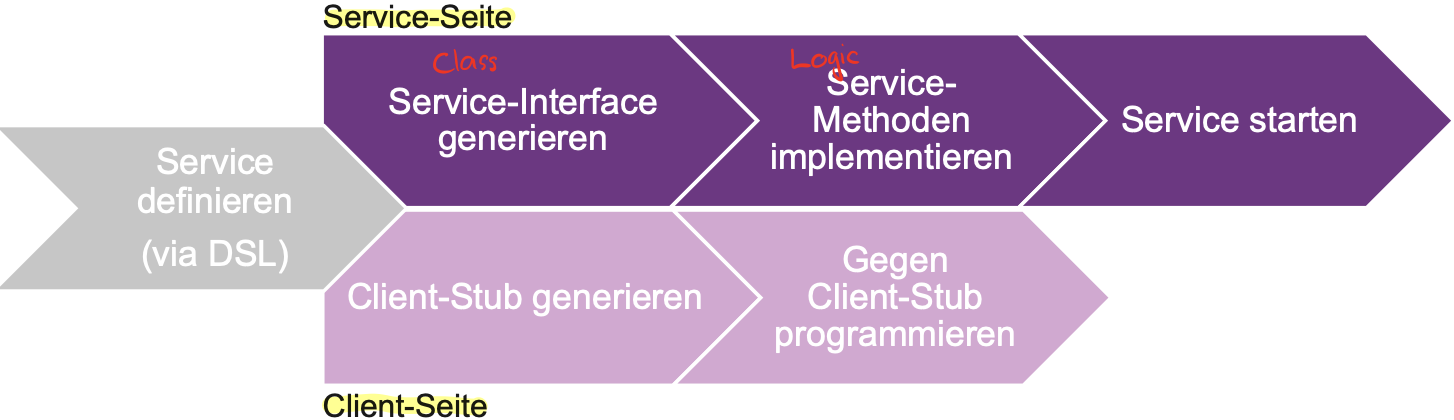
\includegraphics[scale=.27]{graphic/gprc/Developer Workflow.png}
\end{center}
\vspace{-8pt}


\subsection{Architektur}
\subsubsection{Überblick}
\begin{center}
    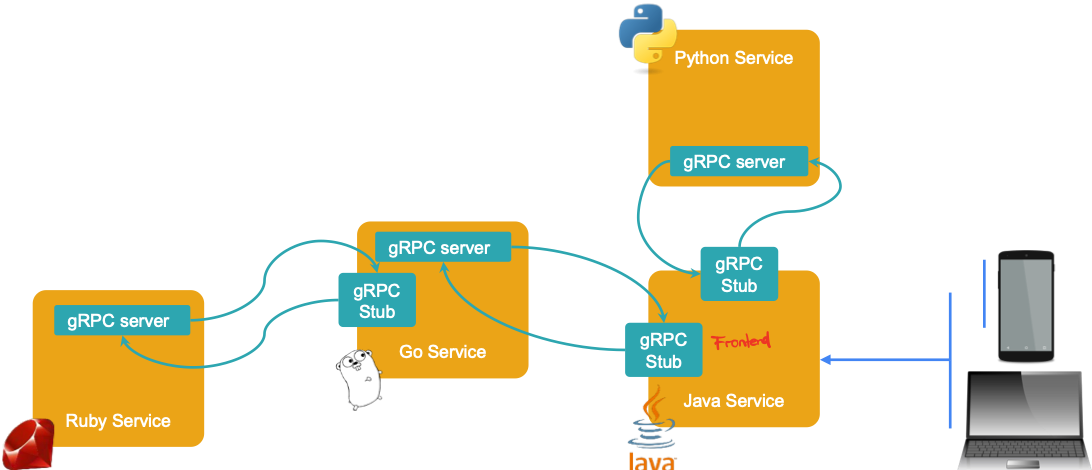
\includegraphics[scale=.35]{graphic/gprc/Systembeispiel.png}
\end{center}
\vspace{-8pt}

\subsubsection{Aufbau \& Kommunikation}
\begin{center}
    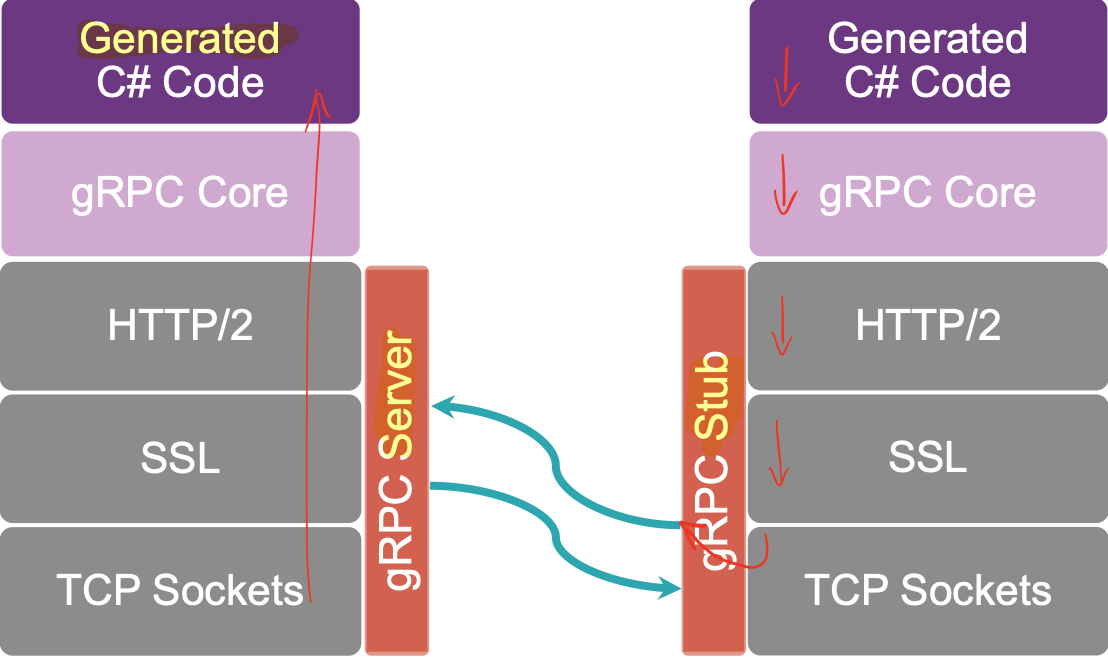
\includegraphics[scale=.3]{graphic/gprc/aufbau.png}
\end{center}
\vspace{-8pt}

\subsubsection{HTTP/2}
\begin{itemize}
    \item Multiplexing
    \begin{itemize}
        \item Mehrere gRPC Calls pro TCP/IP Connection
        \item HTTP/1* benutzte eine TCP/IP pro HTTP Call
        \item Massiv kleinerer Overhead für Disconnect / Reconnect (kleinere Latency)
    \end{itemize}
    \item Bidirectional Streaming
    \begin{itemize}
        \item Asynchrones, Nicht-blockierendes Senden und Empfangen von Streams
        \item Senden und Empfangen parallel möglich
    \end{itemize}
    \item HTTPS
    \begin{itemize}
        \item basieren voll auf HTTPS
    \end{itemize}
    \item Header Compression
\end{itemize}

\subsubsection{HTTP/2 Request and Response Multiplexing}
\begin{center}
    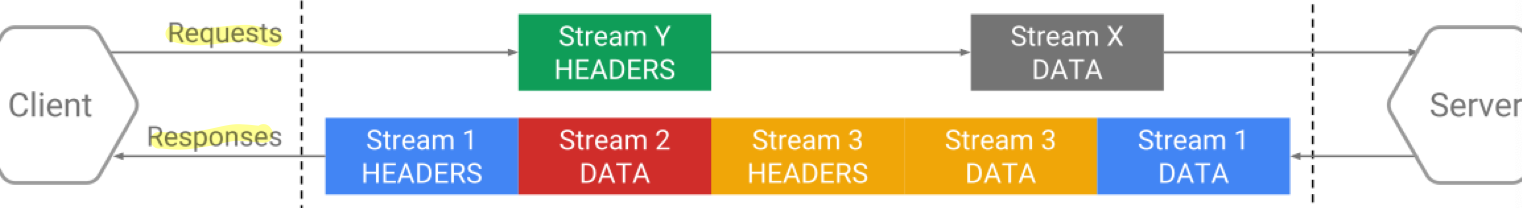
\includegraphics[scale=.3]{graphic/gprc/req resp.png}
\end{center}
\vspace{-8pt}
Performance-Unterschied zw. HTTP/1.1 zu HTTP/2hauptsächlich wegen Multiplexing

\subsubsection{Beispiel / Service}
\begin{center}
    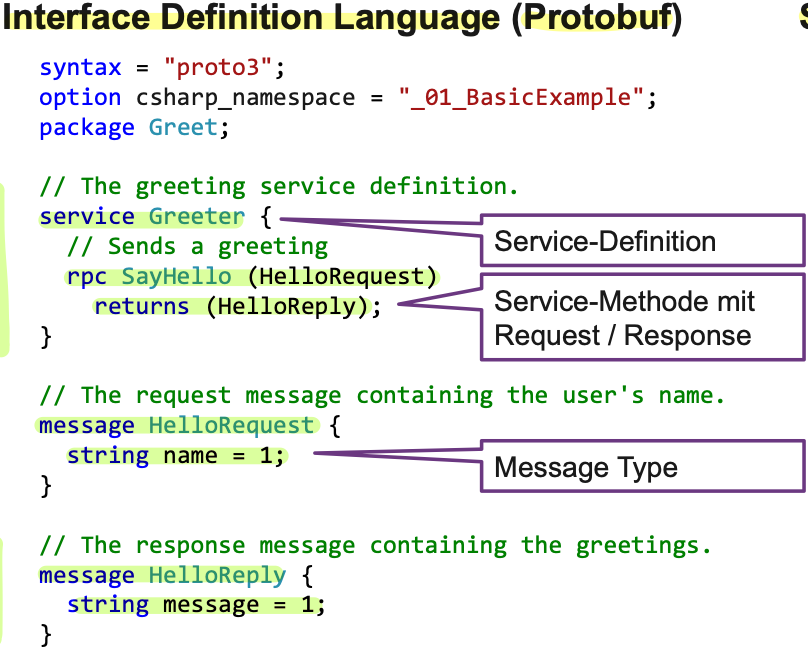
\includegraphics[scale=.39]{graphic/gprc/bsp service 1.png}
    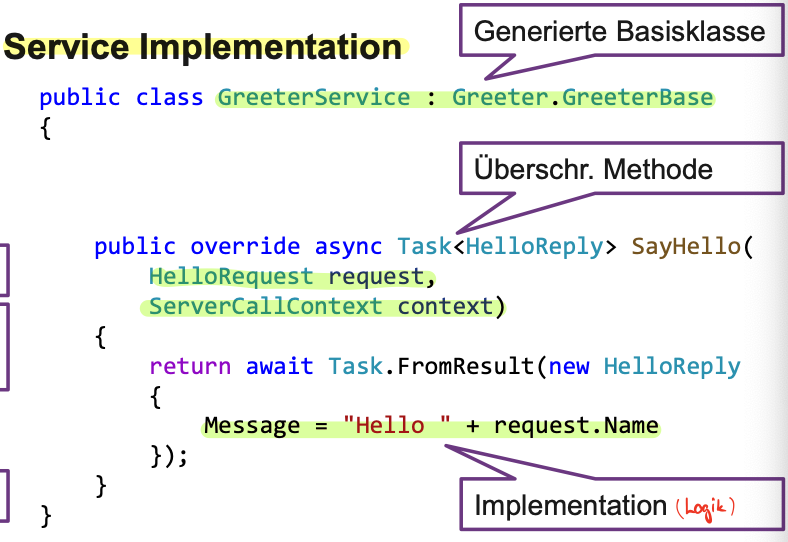
\includegraphics[scale=.39]{graphic/gprc/bsp service 2.png}
\end{center}
\vspace{-8pt}
\subsubsection{Beispiel / Client}
\begin{center}
    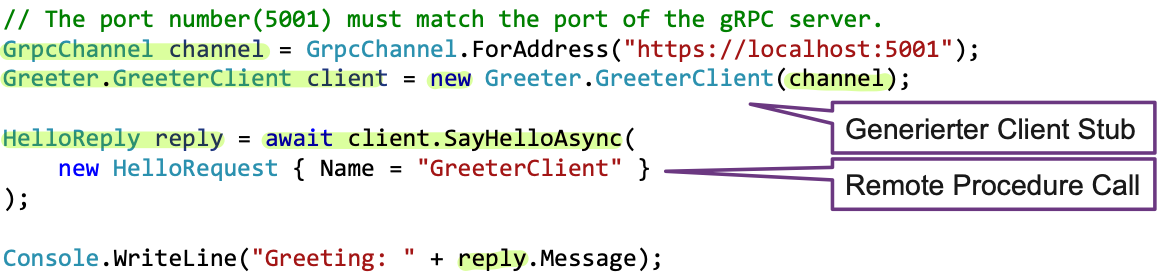
\includegraphics[scale=.42]{graphic/gprc/bsp service client.png}
\end{center}
\vspace{-8pt}

\subsubsection{Vergleich gRPC / REST}
\begin{center}
    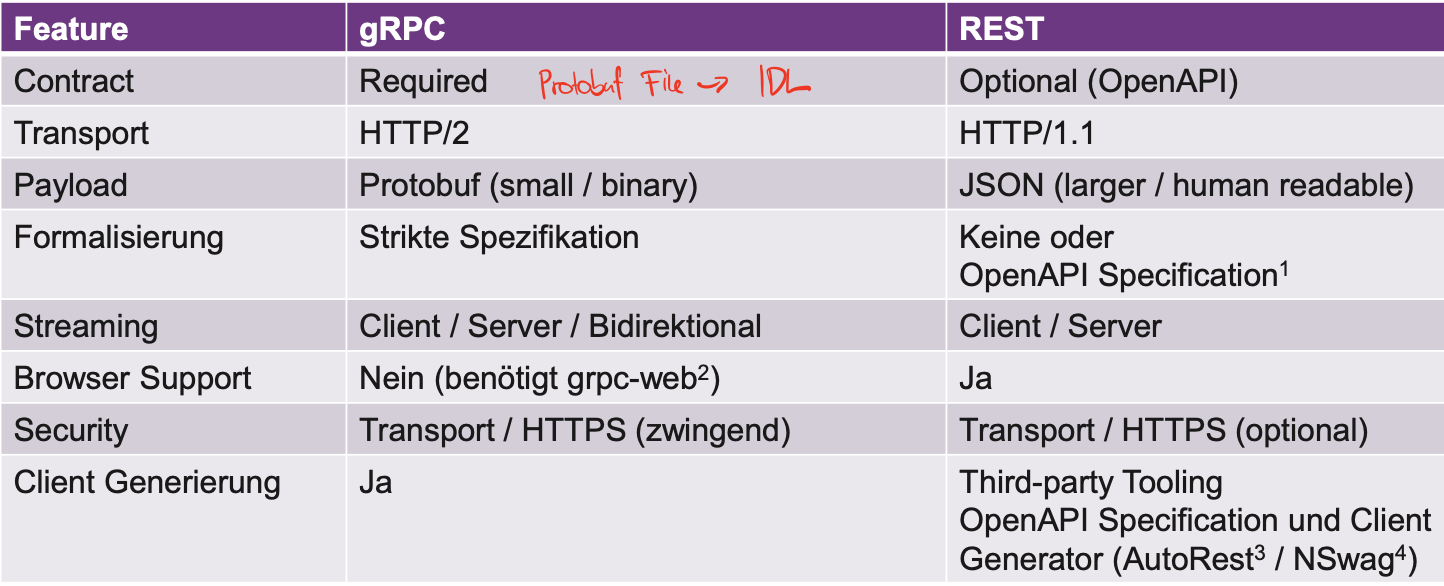
\includegraphics[scale=.3]{graphic/gprc/Vergleich gRPC REST.png}
\end{center}
\vspace{-8pt}

\subsection{Protocol Buffers}
\subsubsection{Umfang}
\begin{itemize}
    \item Interface Definition Language (IDL)
    \begin{itemize}
        \item Eine Subform einer Domain Specific Language (DSL)
        \item Beschreibt ein Service Interface platform- und sprach-neutral
    \end{itemize}
    \item Data Model
    \begin{itemize}
        \item Beschreibt Messages resp. Request- und Response-Objekte
    \end{itemize}
    \item Wire Format
    \begin{itemize}
        \item Beschreibt das Binärformat zur Übertragung
    \end{itemize}
    \item Serialisierungs- / Deserialisierungs-Mechanismen
    \item Service-Versionierung
\end{itemize}

\subsubsection{Proto Files}
\begin{center}
    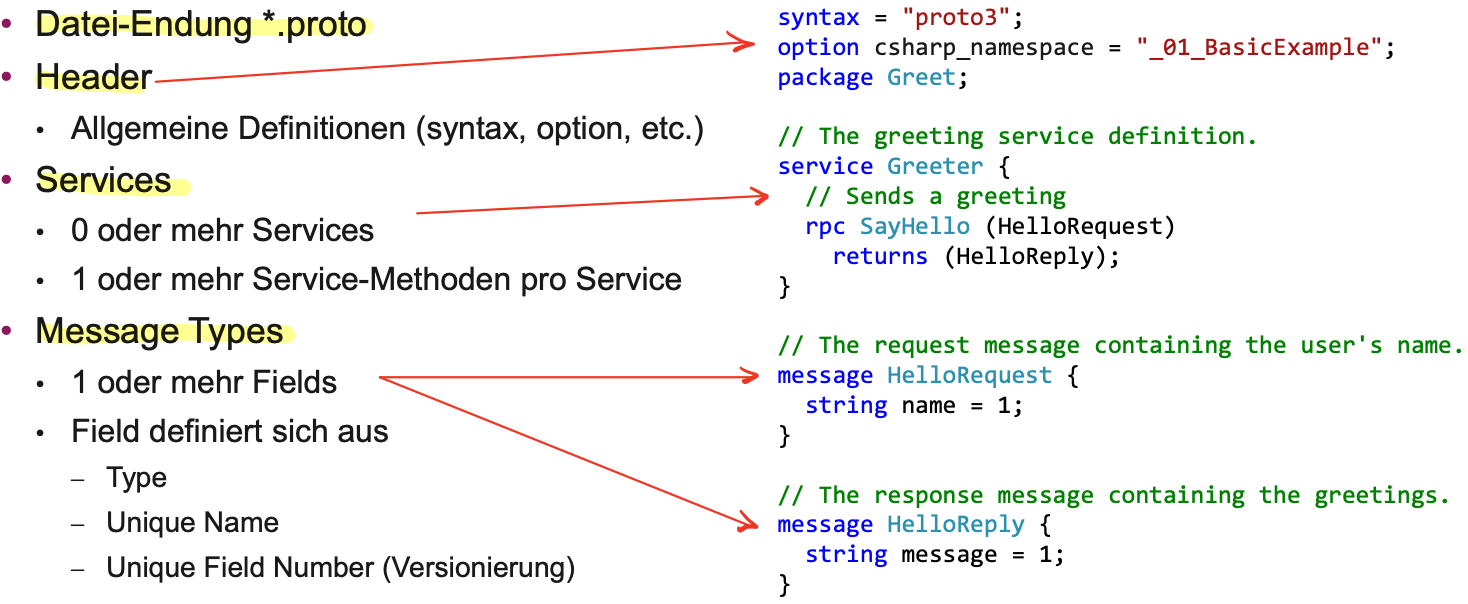
\includegraphics[scale=.35]{graphic/gprc/Proto Files.png}
\end{center}
\vspace{-8pt}

\subsubsection{Messages / Fields}
\begin{center}
    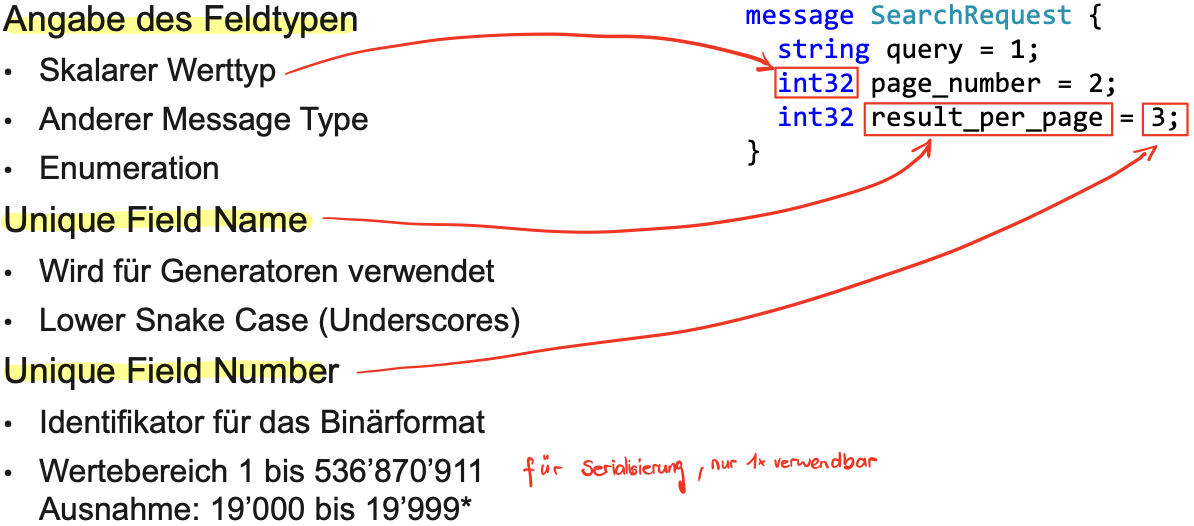
\includegraphics[scale=.35]{graphic/gprc/Messages Fields.png}
\end{center}
\vspace{-8pt}

\subsubsection{Fields / Repeated Fields}
\begin{center}
    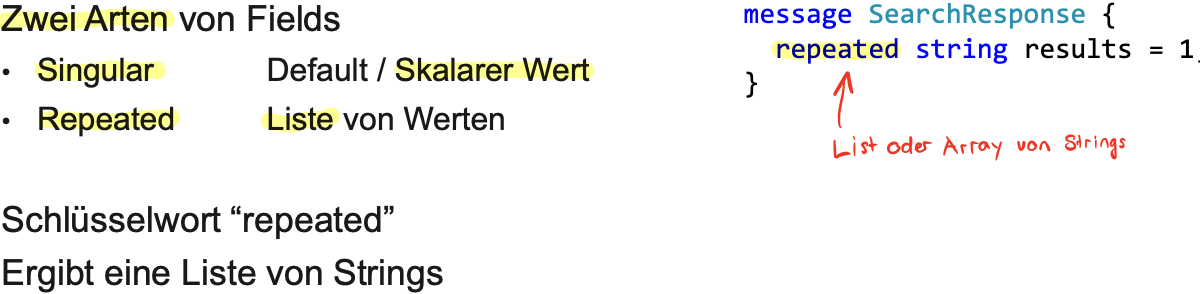
\includegraphics[scale=.35]{graphic/gprc/Fields Repeated Fields.png}
\end{center}
\vspace{-8pt}

\subsubsection{Enumerations}
\begin{center}
    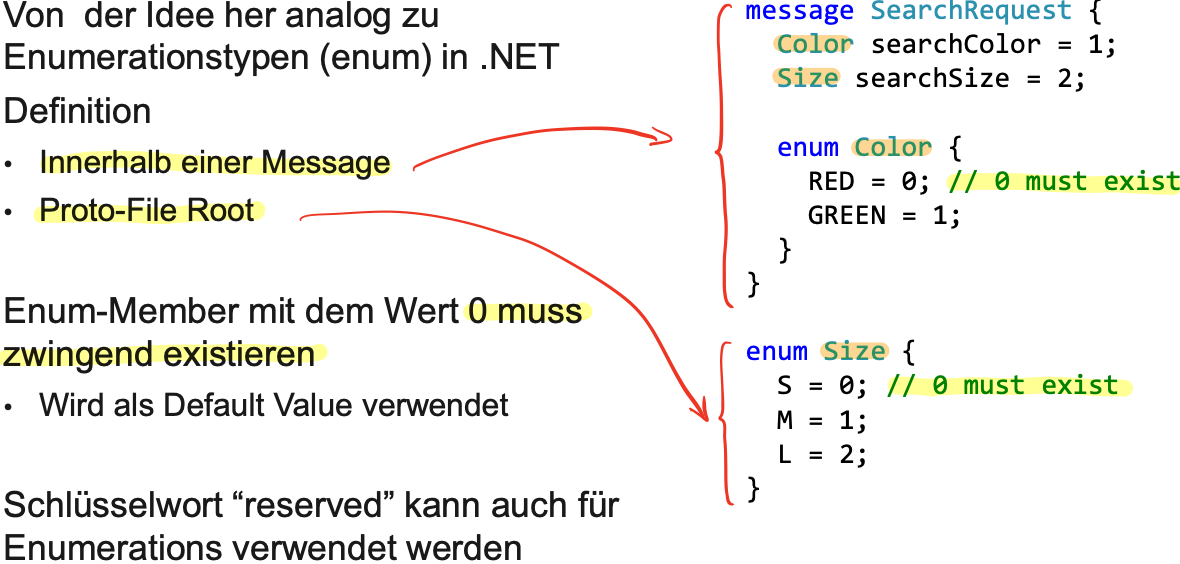
\includegraphics[scale=.35]{graphic/gprc/Enumerations.png}
\end{center}
\vspace{-8pt}

\subsubsection{Message Type Composition \& Imports}
\begin{center}
    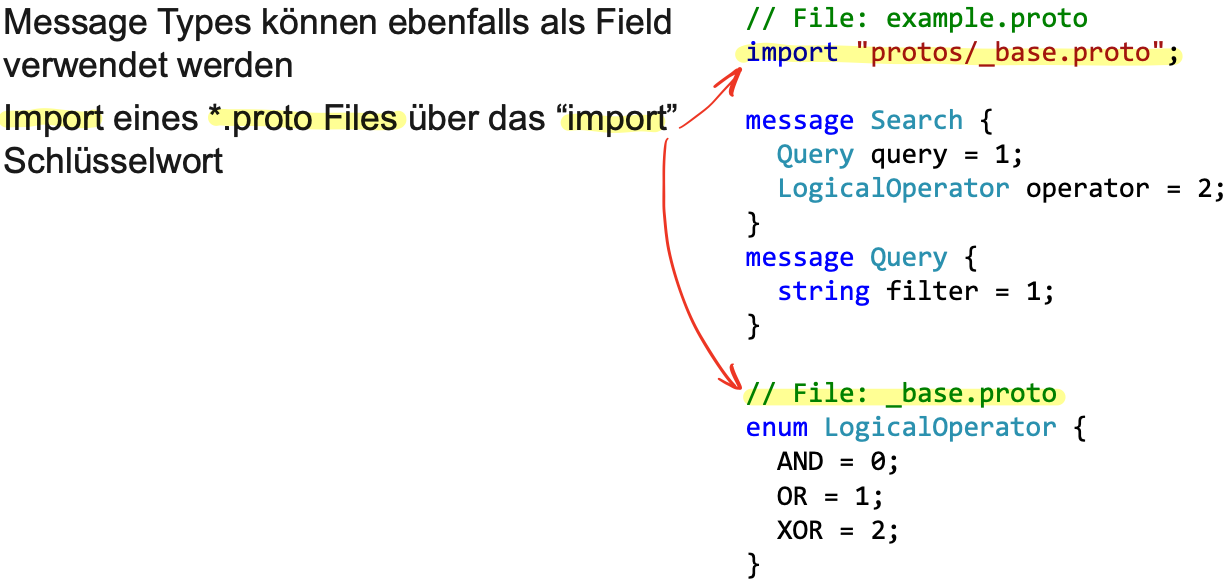
\includegraphics[scale=.35]{graphic/gprc/Message Type Composition Imports.png}
\end{center}
\vspace{-8pt}

\subsubsection{Reserved Fields}
\begin{center}
    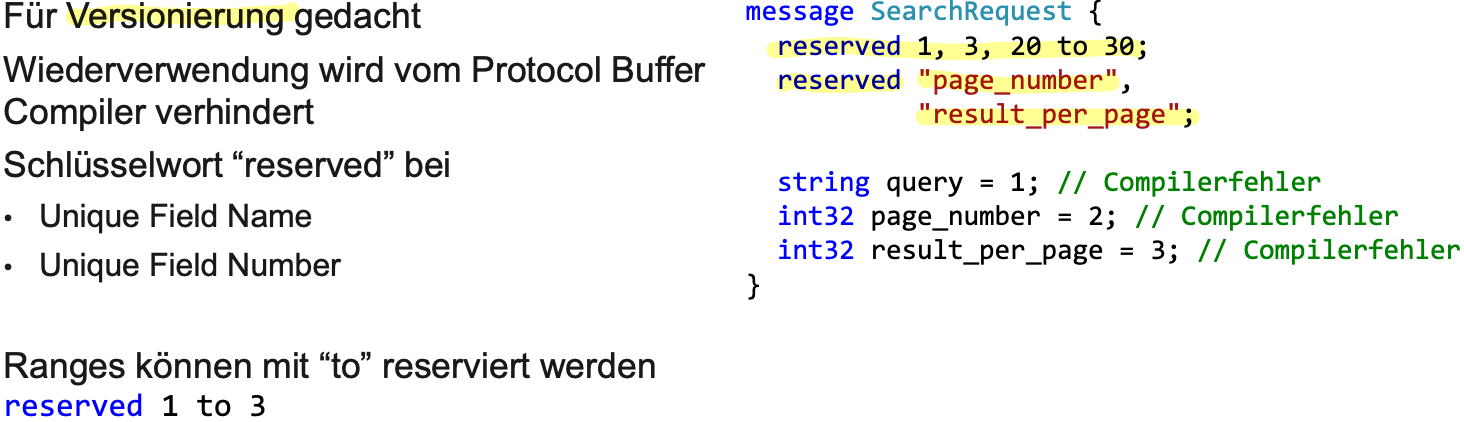
\includegraphics[scale=.34]{graphic/gprc/reserved fields.png}
\end{center}
\vspace{-8pt}

\subsection{gRPC C \# API}
\subsubsection{C\# API / Startup}
\begin{center}
    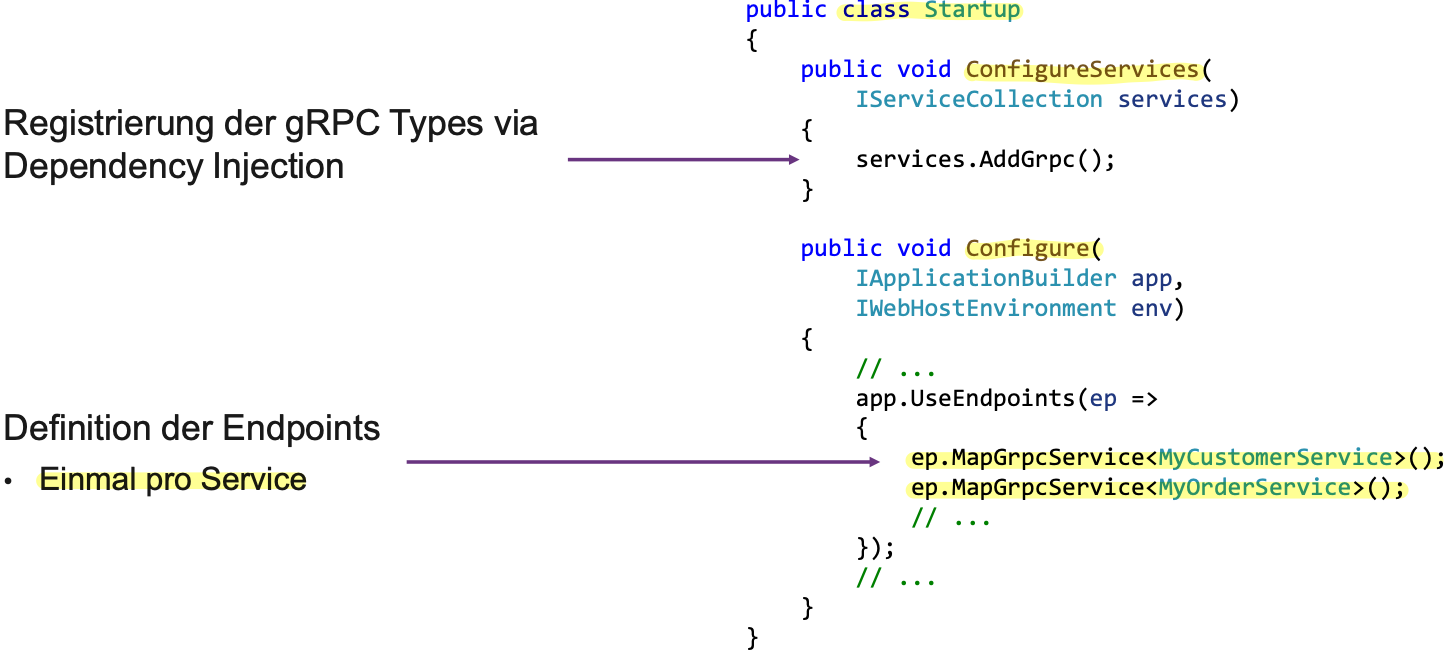
\includegraphics[scale=.35]{graphic/gprc/api start.png}
\end{center}
\vspace{-8pt}


\subsection{Streams}
\begin{itemize}
    \item Unterstützt drei Modi
    \begin{itemize}
        \item Server Streaming Call
        \item Client Streaming Call
        \item Duplex Streaming Call
    \end{itemize}
    \item Reliability:
    \begin{itemize}
        \item End-to-end Reliability $\rightarrow$ Garantiertes Ausliefern der Nachrichten gewährleistet
        \item Ordered Delivery $\rightarrow$ Reihenfolge gewährleistet
    \end{itemize}
\end{itemize}

\subsubsection{Synchrones Lesen}
\begin{center}
    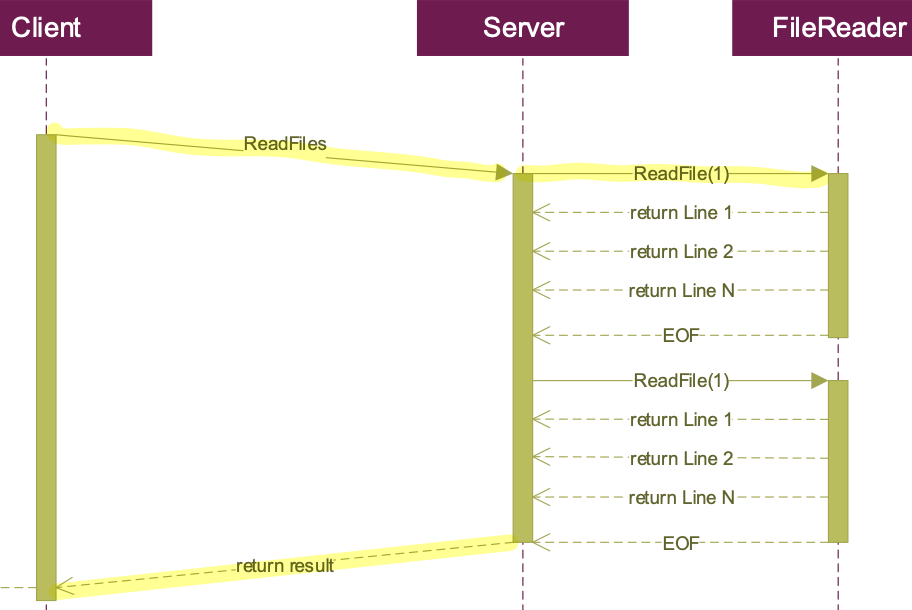
\includegraphics[scale=.35]{graphic/gprc/Synchrones Lesen.png}
\end{center}
\vspace{-8pt}

\subsubsection{Asynchrones Lesen}
\begin{center}
    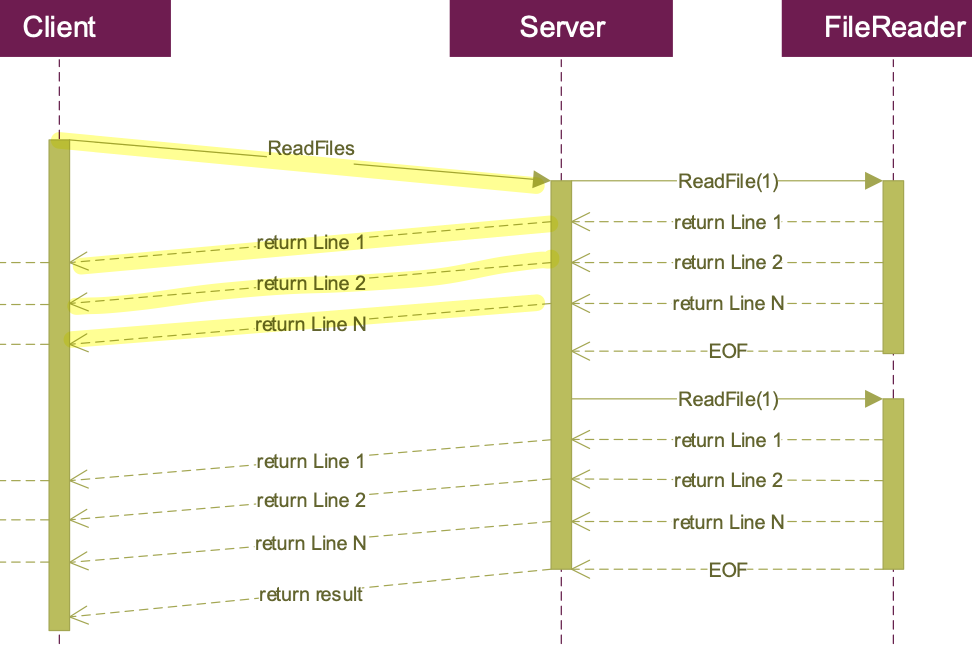
\includegraphics[scale=.35]{graphic/gprc/Asynchrones Lesen.png}
\end{center}
\vspace{-8pt}

\subsubsection{Protocol Buffers}
\begin{center}
    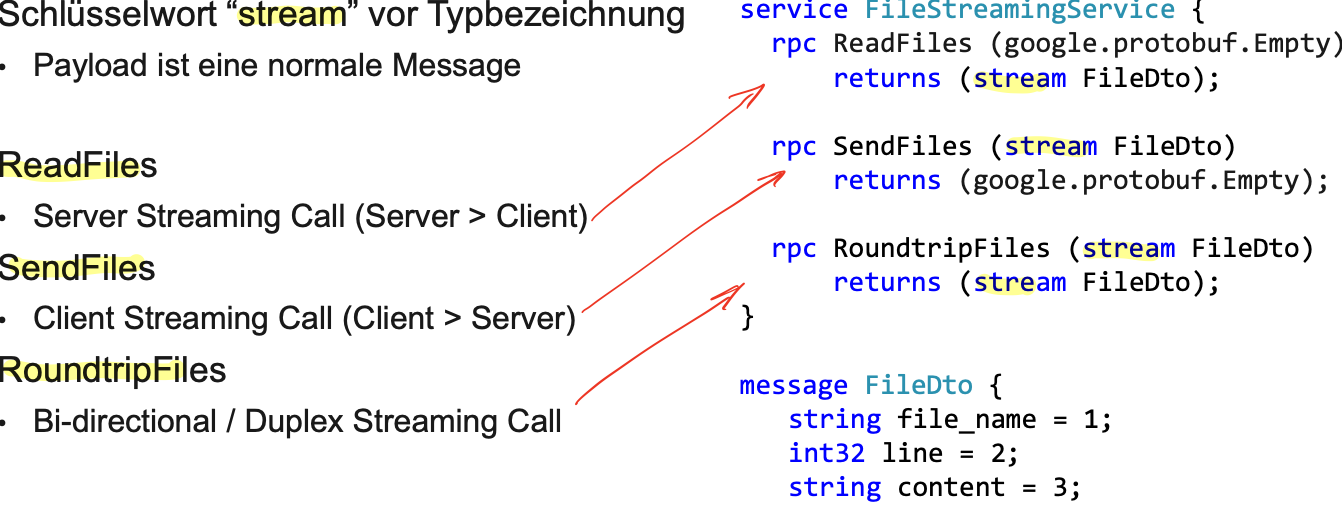
\includegraphics[scale=.35]{graphic/gprc/Protocol Buffers.png}
\end{center}
\vspace{-8pt}

\subsubsection{Server Streaming Call (Server $\rightarrow$ Client)}
\paragraph{Client}
\begin{center}
    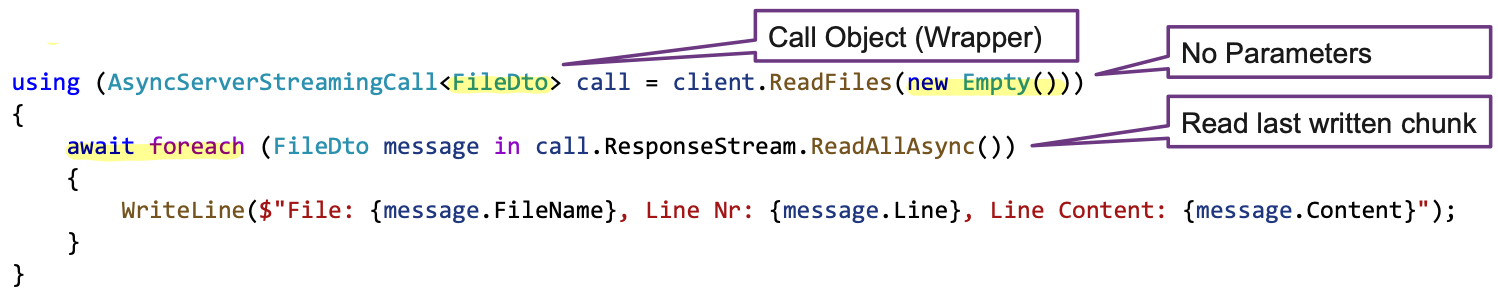
\includegraphics[scale=.33]{graphic/gprc/Server Streaming Call client.png}
\end{center}
\vspace{-8pt}
\paragraph{Server}
\begin{center}
    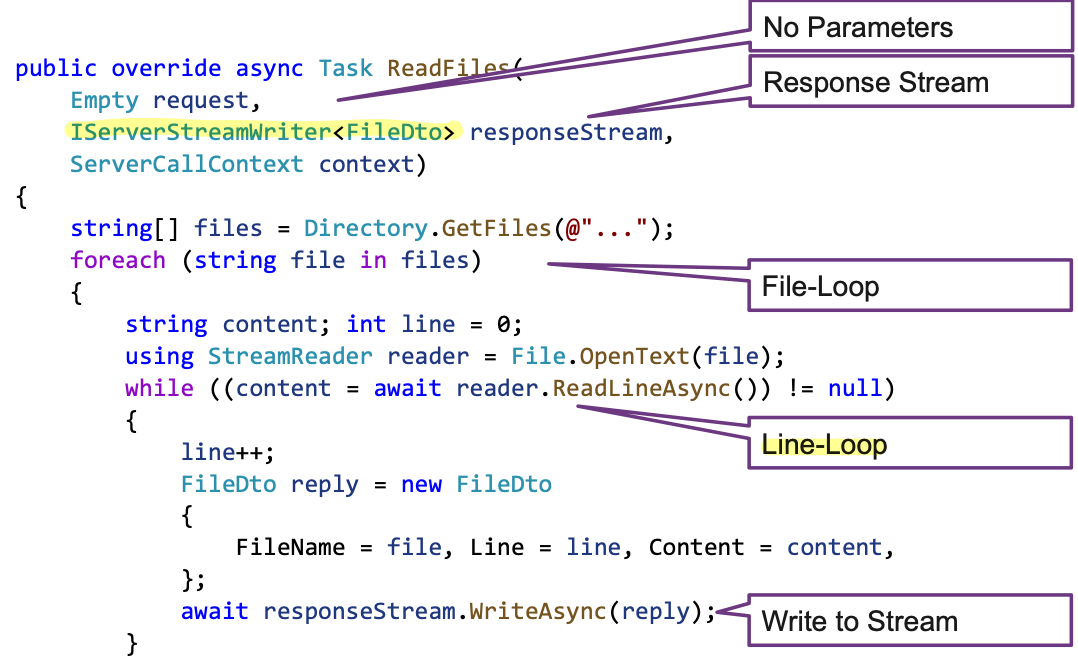
\includegraphics[scale=.4]{graphic/gprc/Server Streaming Call Service.png}
\end{center}
\vspace{-8pt}

\subsubsection{Client Streaming Call (Client $\rightarrow$ Server)}
\paragraph{Client}
\begin{center}
    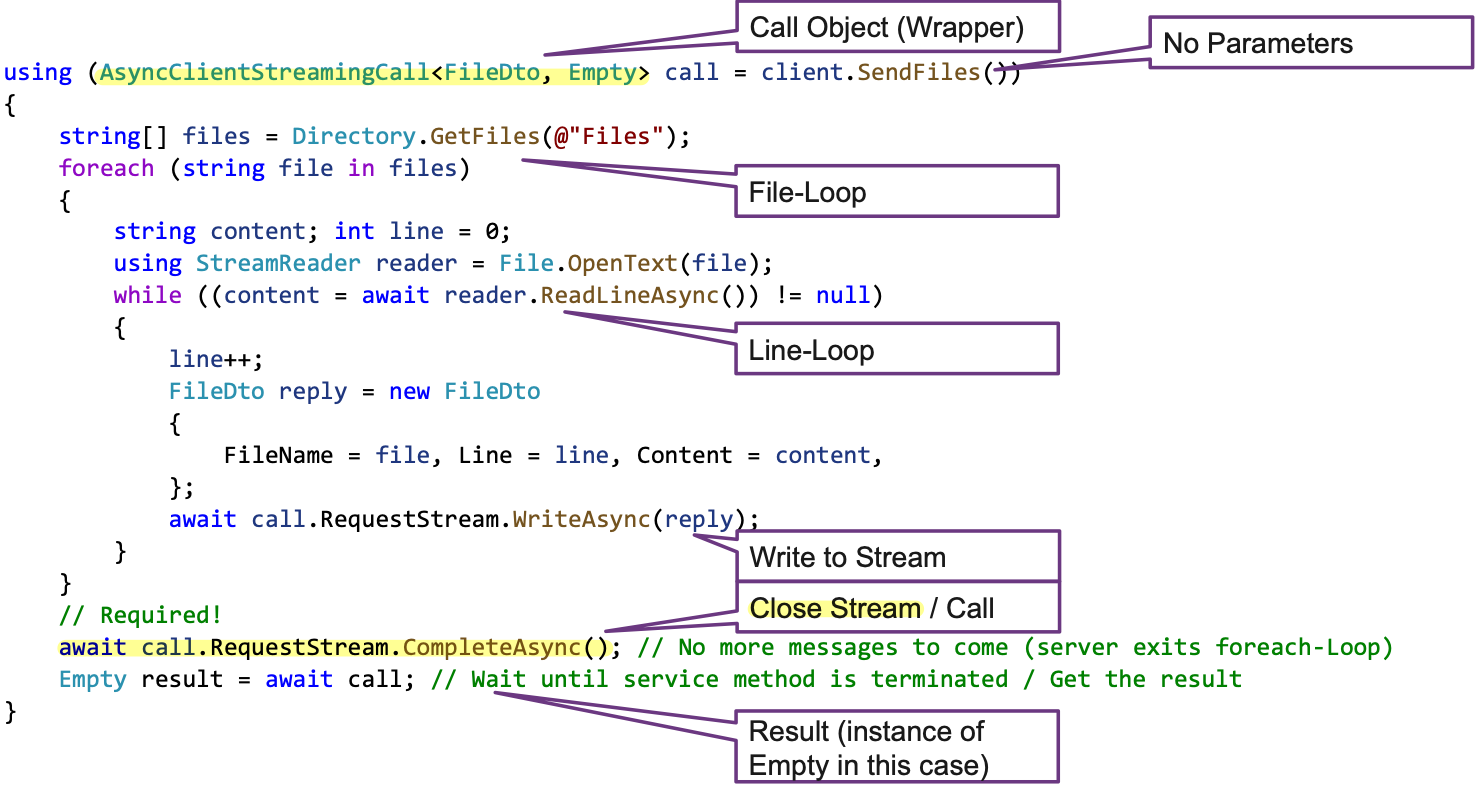
\includegraphics[scale=.39]{graphic/gprc/Client Streaming Call client.png}
\end{center}
\vspace{-8pt}
\paragraph{Server}
\begin{center}
    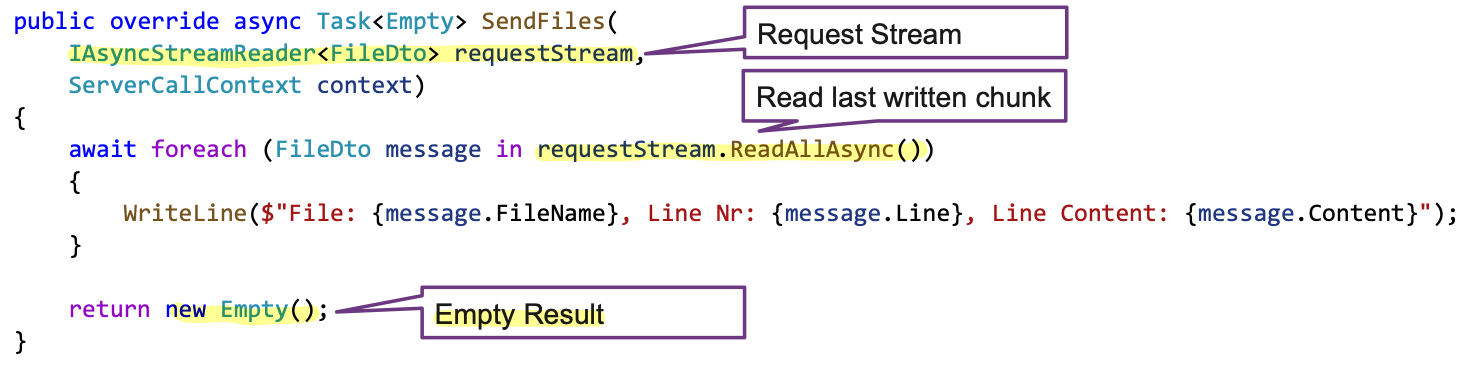
\includegraphics[scale=.38]{graphic/gprc/Client Streaming Call service.png}
\end{center}
\vspace{-8pt}

\subsubsection{Bi-directional (Duplex) (Client $\rightarrow$ Server $\rightarrow$ Client)}
\paragraph{Client}
\begin{center}
    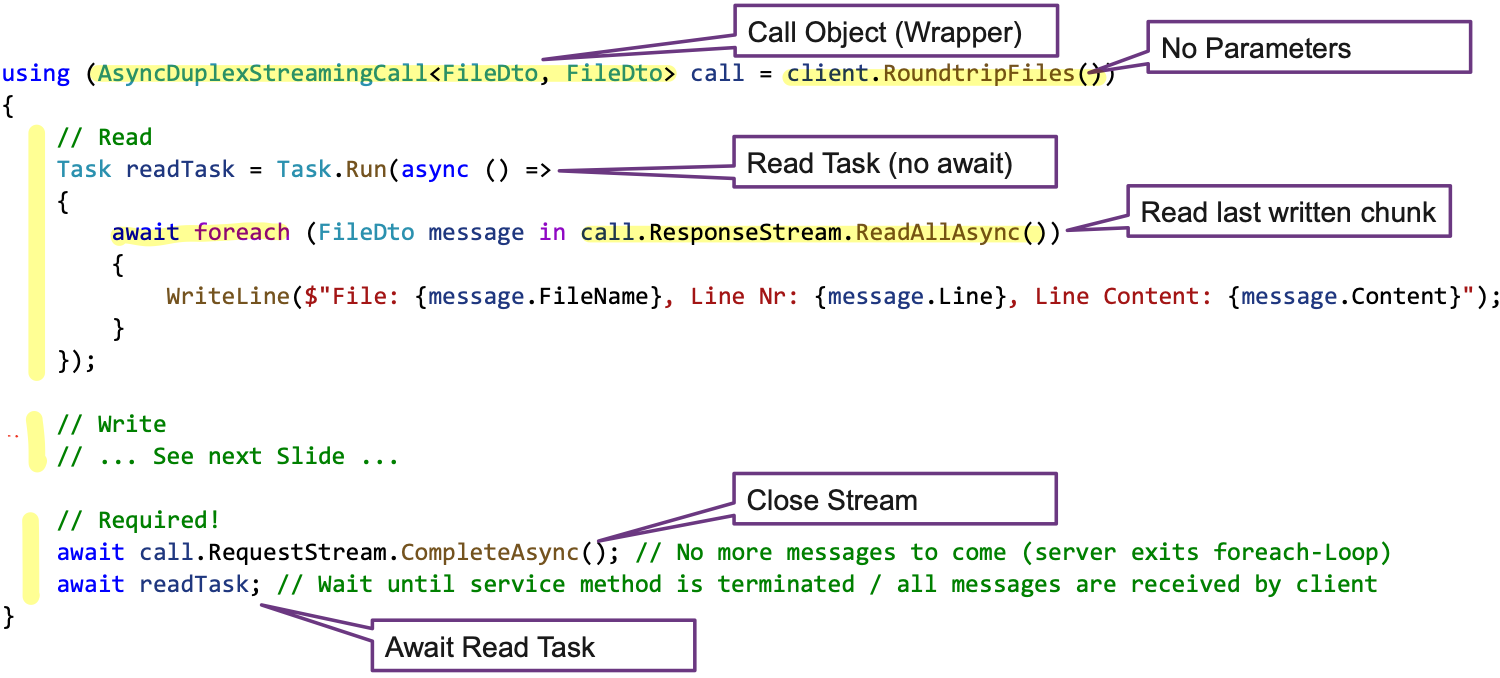
\includegraphics[scale=.34]{graphic/gprc/Bi-directional client1.png}
    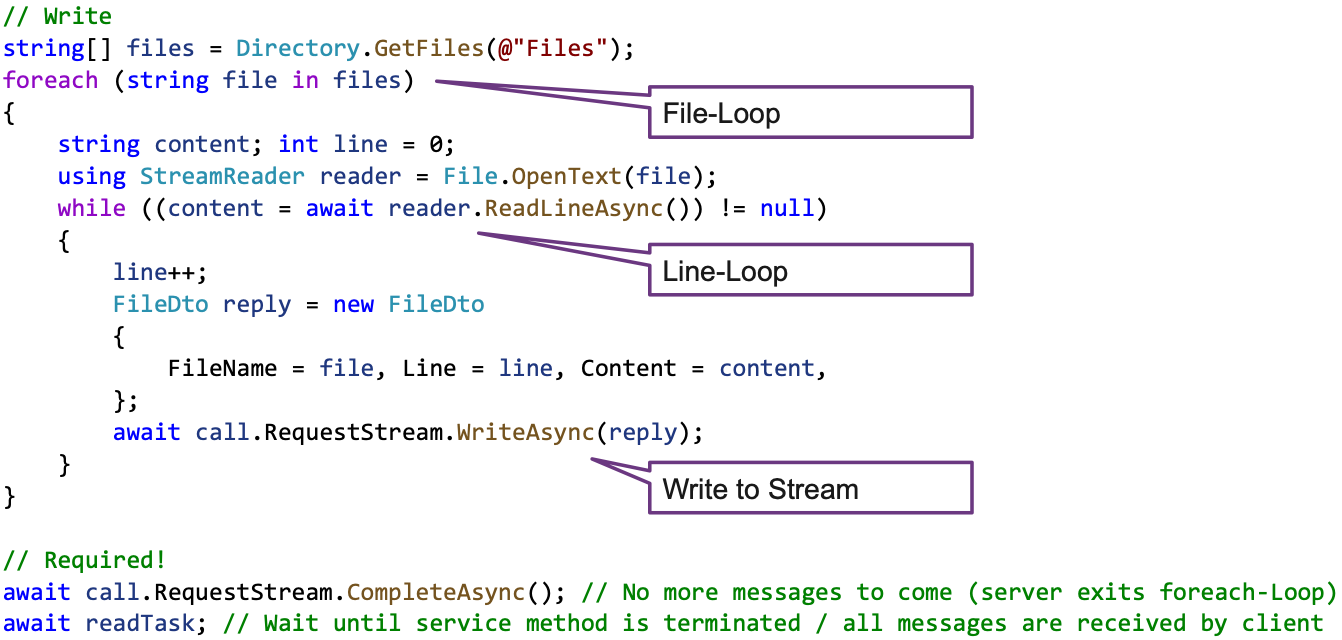
\includegraphics[scale=.34]{graphic/gprc/Bi-directional client2.png}
\end{center}
\vspace{-8pt}
\paragraph{Server}
\begin{center}
    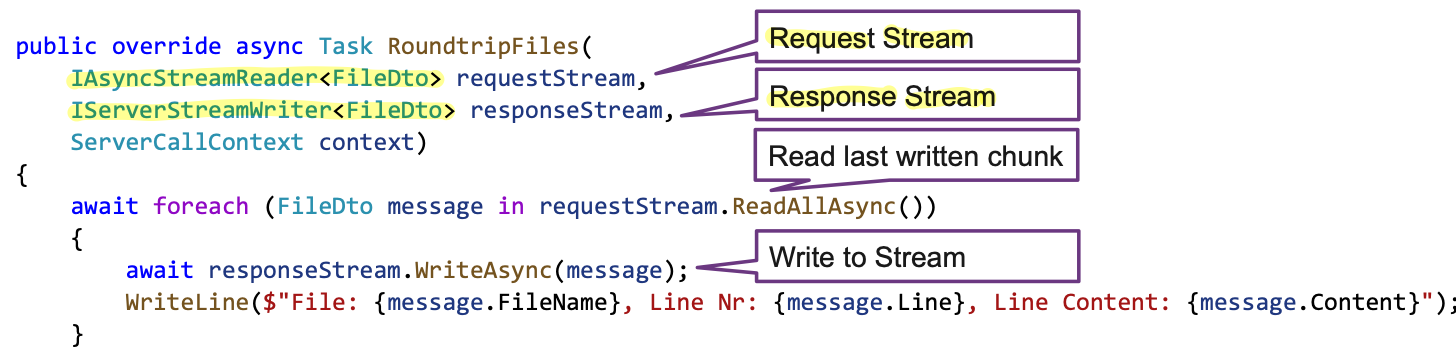
\includegraphics[scale=.34]{graphic/gprc/Bi-directional service.png}
\end{center}
\vspace{-8pt}


\subsection{Exception Handling}
Grundsätzlich immer via RpcException! $\rightarrow$ Basierend auf StatusCodes

\subsubsection{Status Codes}
\begin{center}
    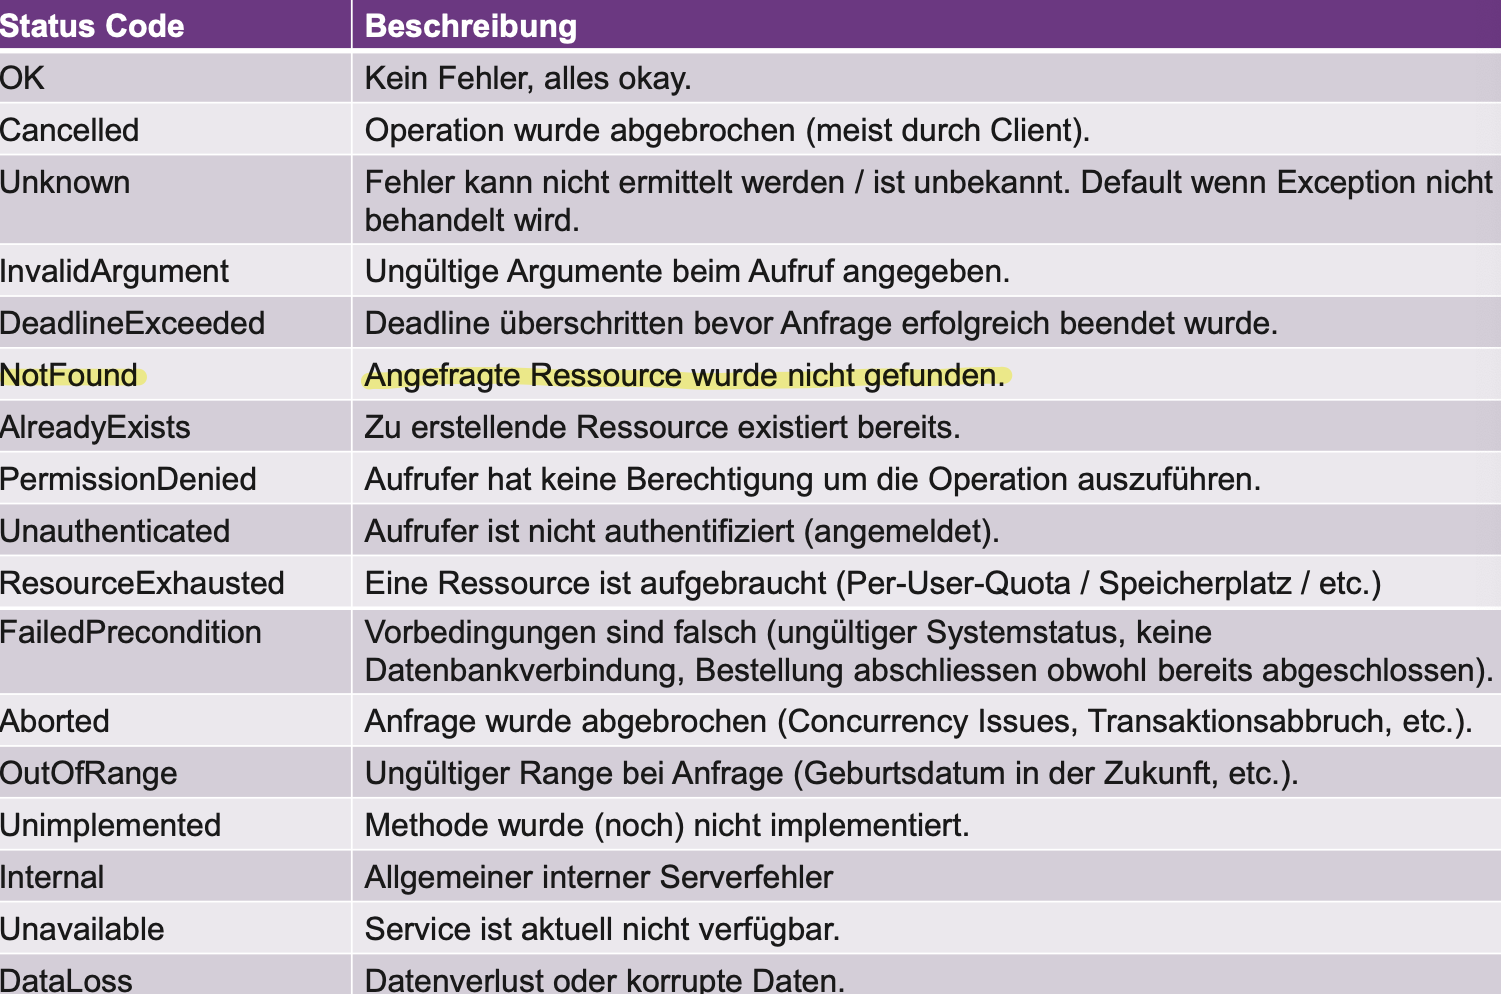
\includegraphics[scale=.3]{graphic/gprc/Status Codes.png}
\end{center}
\vspace{-8pt}

\subsubsection{Unbehandelte Exception}
Exception wird auf Server nicht sauber behandelt
\begin{itemize}
    \item Server Runtime fängt Exception
    \item Wirft RpcException
    \item Status Code “Unknown”
\end{itemize}
\begin{lstlisting}
public override async Task<Empty> Unhandled(
    Empty request,
    ServerCallContext context)
{
    throw new Exception("Unhandled Exception");
}
\end{lstlisting}

\subsubsection{Behandelte Exception}
Exception wird auf Server sauber behandelt und korrekt verpackt
\begin{lstlisting}
public override async Task<Empty> NotFound(
    Empty request,
    ServerCallContext context)
{
    throw new RpcException(
        new Status(
            StatusCode.NotFound,
            "Something was not found."
));}
\end{lstlisting}


\subsection{Special Types}
\subsubsection{Empty}
Platzhalter für Null-Werte
\begin{lstlisting}
Empty e = new Empty();
\end{lstlisting}

\subsubsection{Timestamp}
UTC Zeitstempel
\begin{lstlisting}
Timestamp ts = new Timestamp {
    // Seconds since 1970-01-01T00:00:00Z 
    Seconds = DateTime.UtcNow.Second
};
\end{lstlisting}

\subsubsection{Bytes / ByteString}
Binärer Datentyp
\begin{lstlisting}
// Empty ByteString
ByteString bs = ByteString.Empty;

// To ByteStream
bs = ByteString.CopyFromUtf8("X");
\end{lstlisting}

\subsubsection{Collections: Repeated Fields}
Generiert ein Repeated Field Property $\rightarrow$ read only!
\begin{lstlisting}
message RepeatedResponse {
repeated string results = 1; }
\end{lstlisting}

\subsubsection{Collections: Map Fields}
Generiert ein Map Field Property $\rightarrow$ read only!
\begin{lstlisting}
message MapResponse {
map<int32, string> results = 1; }
\end{lstlisting}

\subsubsection{Oneof}
Lässt eine Auswahl von Typen zu
\begin{lstlisting}
message OneofResponse {
    oneof results {
        string image_url = 1;
        bytes image_data = 2;
    }}
\end{lstlisting}
\subsubsection{Any}
Repräseniert einen beliebigen Wert
\begin{lstlisting}
var response = new AnyResponse();

// Pack (message type)
response.Results = Any.Pack(new CustomerResponse());
\end{lstlisting}


\subsection{Configuration / Logging}
\subsubsection{Server Konfiguration}
\begin{center}
    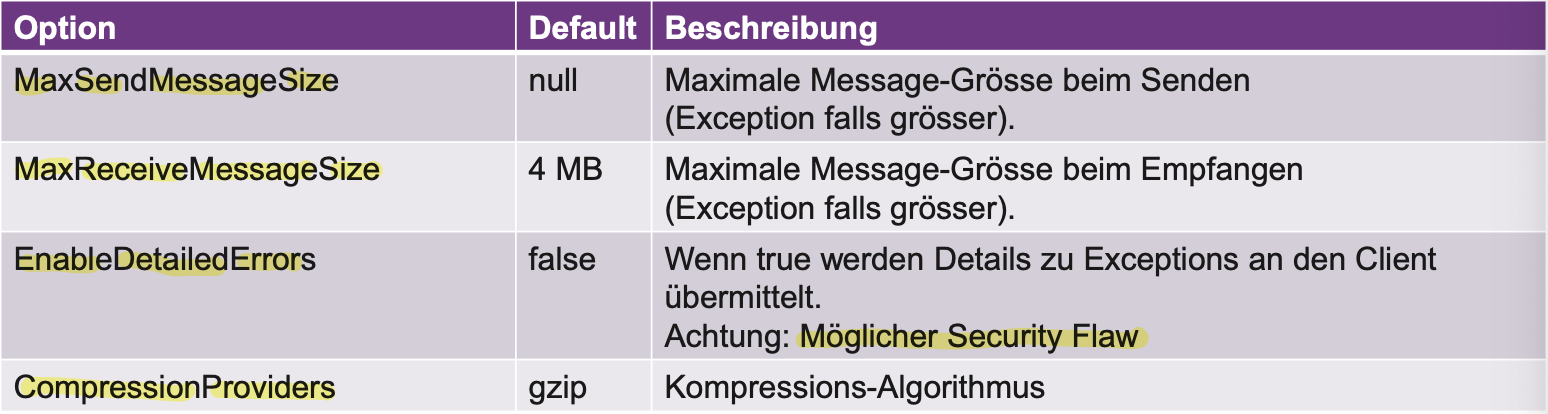
\includegraphics[scale=.28]{graphic/gprc/Server Konfiguration.png}
    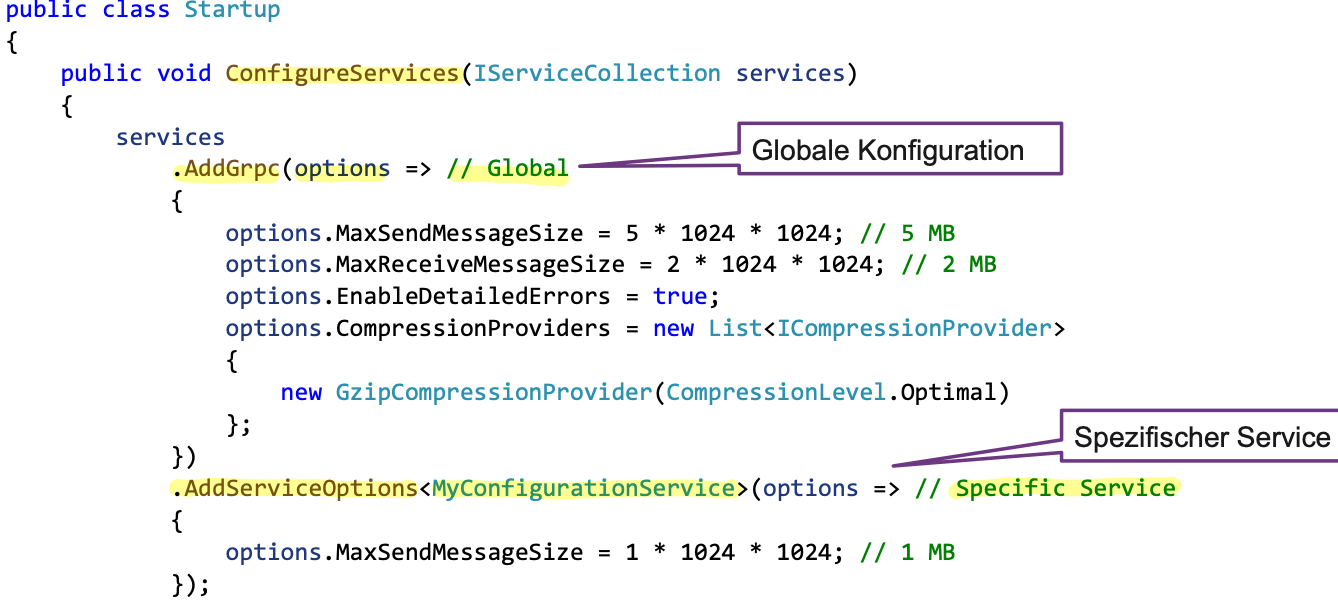
\includegraphics[scale=.4]{graphic/gprc/Server Konfiguration2.png}
\end{center}
\vspace{-8pt}

\subsubsection{Client Konfiguration}
\begin{center}
    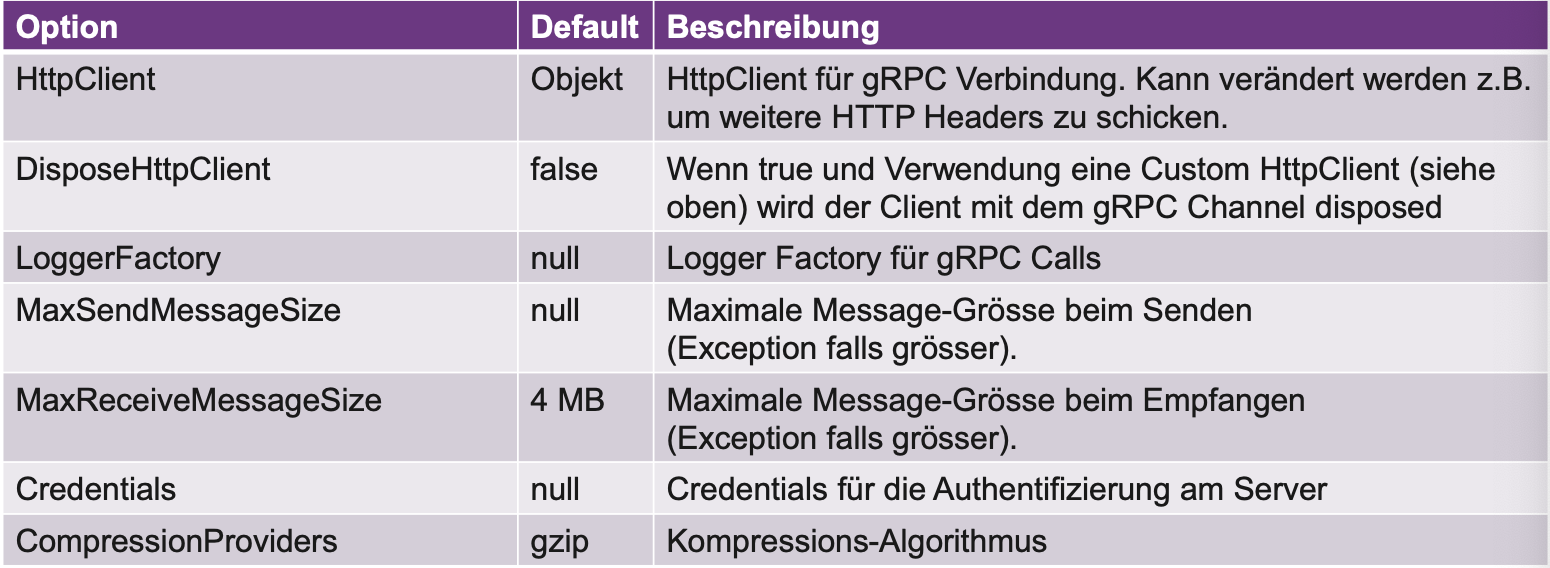
\includegraphics[scale=.28]{graphic/gprc/Client Konfiguration1.png}
    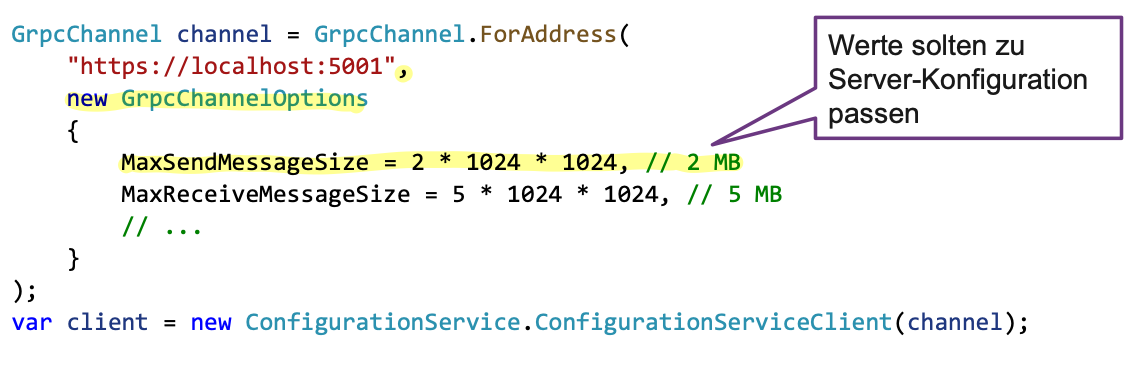
\includegraphics[scale=.4]{graphic/gprc/Client Konfiguration2.png}
\end{center}
\vspace{-8pt}

\subsubsection{Server-side Logging (2 Varianten)}
\begin{center}
    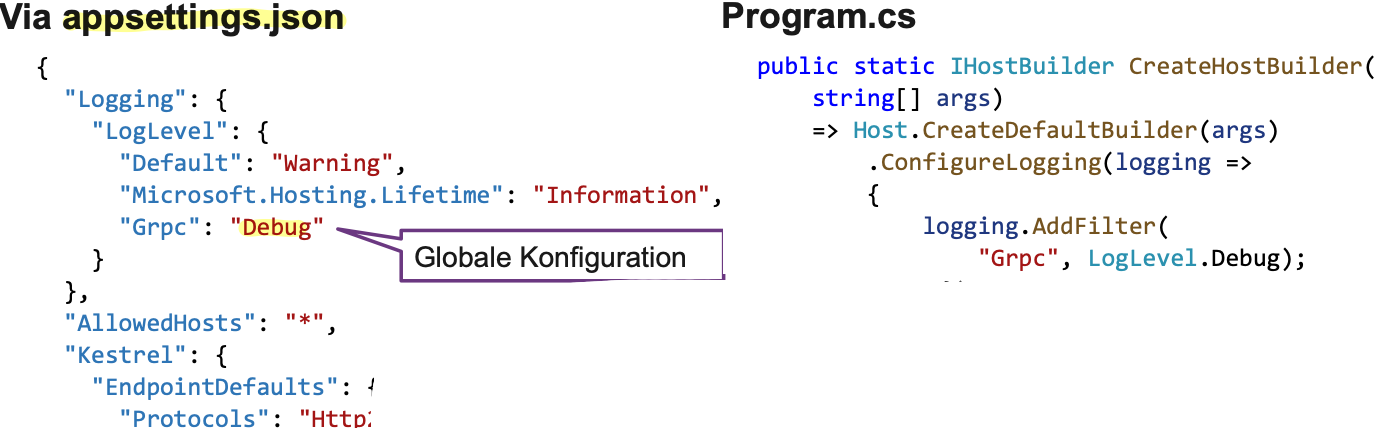
\includegraphics[scale=.38]{graphic/gprc/log.png}
\end{center}
\vspace{-8pt}


\newpage